\documentclass[aspectratio=169]{beamer}
\usepackage{geometry}

\usetheme{metropolis}           % Use metropolis theme
\usefonttheme[onlymath]{serif}

\usepackage{xeCJK}
%\usepackage{CJKutf8}
\usepackage{graphicx}
\usepackage{amsmath}
\usepackage{multicol}
\usepackage[font=small,labelfont=bf]{caption}
\DeclareCaptionFont{mysize}{\fontsize{7}{9.6}\selectfont}
\captionsetup{font=mysize}

\usepackage{textpos}
\usepackage{adjustbox}
\usepackage{pdfpages}

\newcommand\Fontvi{\fontsize{8}{7.2}\selectfont}

\title{Nders at NTCIR-13 Short Text Conversation }
\author{Han Ni, Liansheng Lin, Ge Xu}
\institute{NetDragon Websoft Inc.}
\date{Dec. 2017}

%\logo{
\includegraphics[height=1.2cm,width=1.35cm]{logo}}

% title page logo
\titlegraphic{\hspace*{11.2cm} 
\includegraphics[height=3cm,width=3.38cm]{logo}
}

\begin{document}
  \maketitle

  % frame title logo
  \addtobeamertemplate{frametitle}{}{%
  \begin{textblock*}{100mm}(.96\textwidth,-1.1cm)
  
\includegraphics[height=1.2cm,width=1.35cm]{logo}
  \end{textblock*}}

    \begin{frame}{System Architecture}
      \begin{figure}
      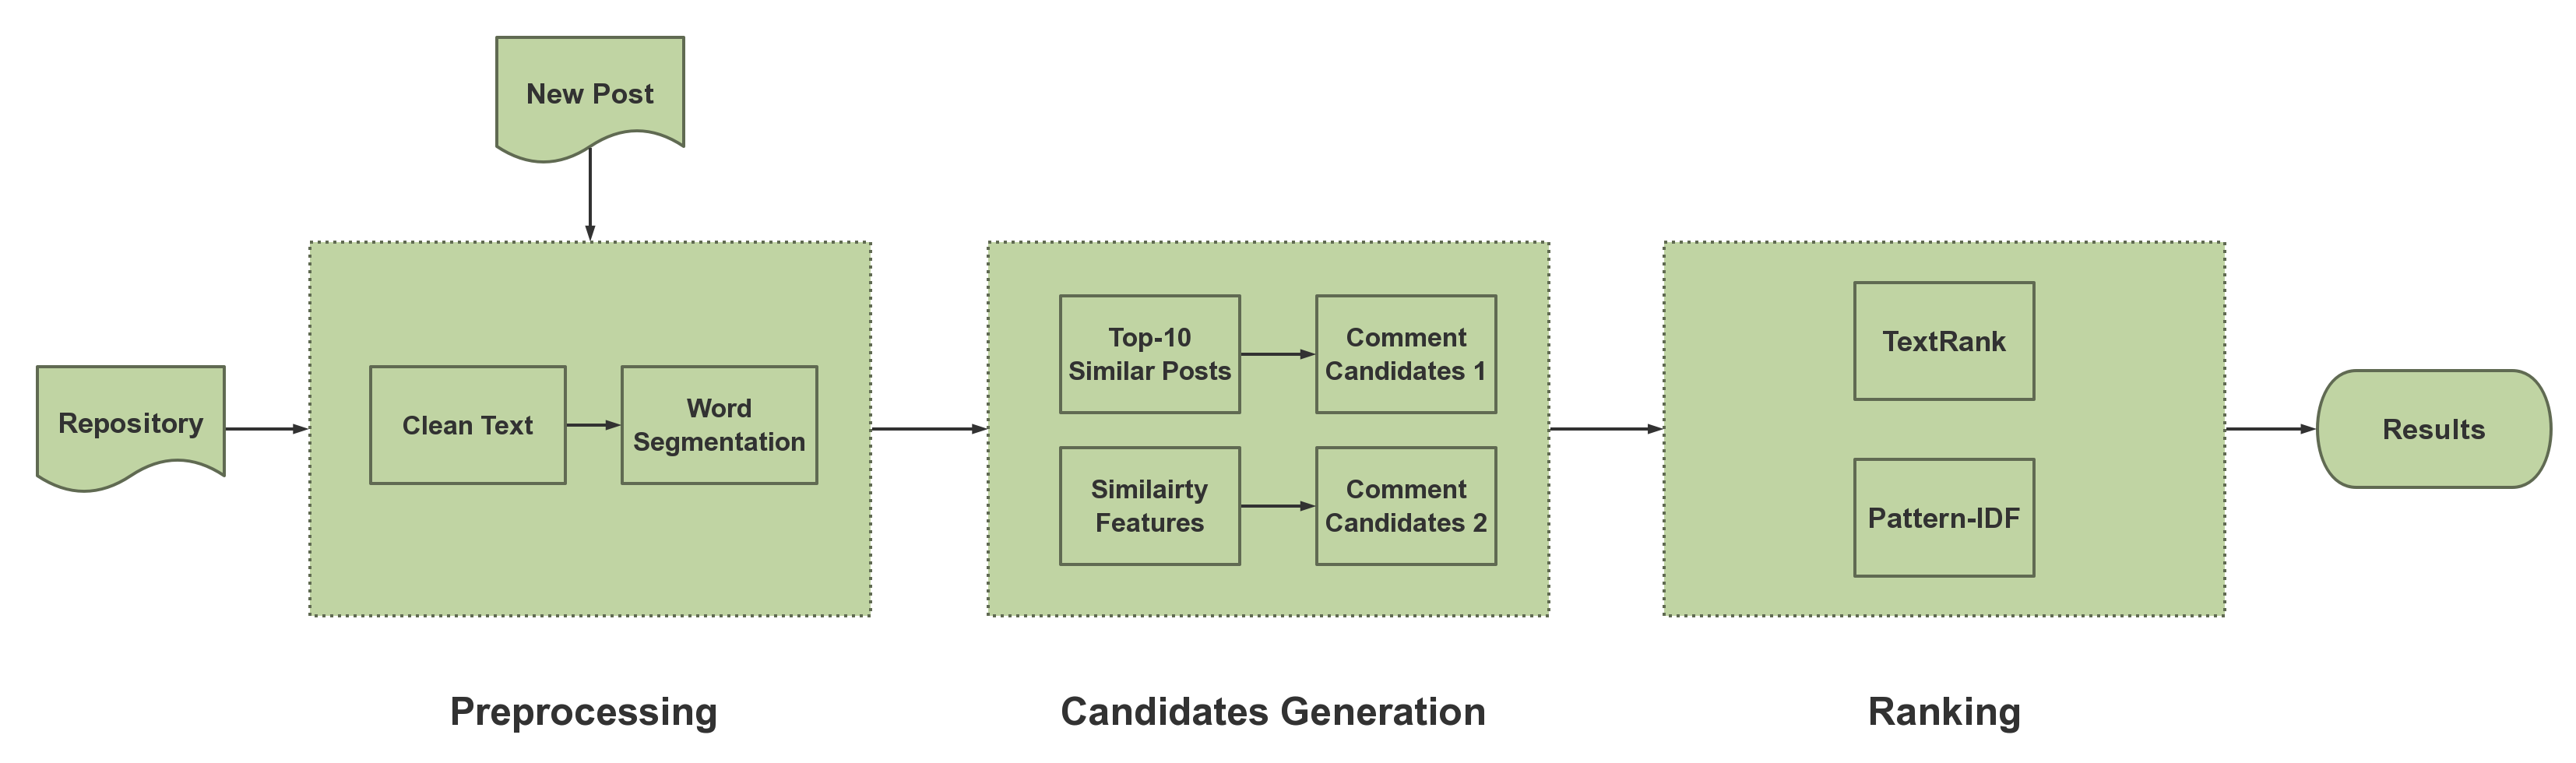
\includegraphics[width=14cm,height=4.63cm]{stc-flow-big.png}
      \caption{System Architecture}
      \end{figure}
    \end{frame}

    \begin{frame}{Preprocessing}
      \begin{itemize}
        \item Traditional-Simplified Chinese conversion
        \item Convert Full-width characters into half-width ones
        \item Word segmentation (PKU standard)
        \item Replace number, time, url with token <\_NUM>, <\_TIME>, <\_URL> respectively
        \item Filter meaningless words and special symbols
      \end{itemize}
    \end{frame}

    {
    \setbeamercolor{background canvas}{bg=}
    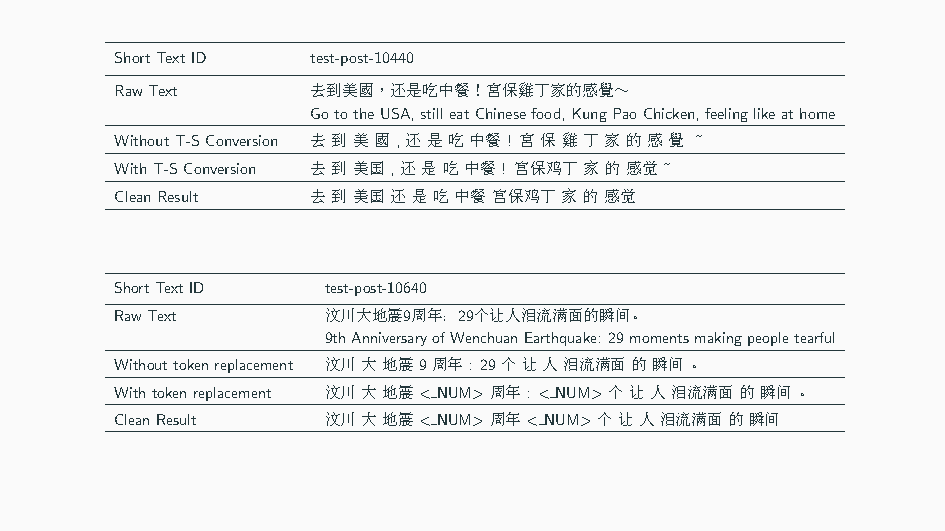
\includepdf[pages=1]{test.pdf}
    }

    

    \begin{frame}{Similarity Features}
      \begin{itemize}
        \item TF-IDF
        \item LSA (Latent Semantic Analysis)
        \item LDA (Latent Dirichlet Allocation)
        \item Word2Vec (skip-gram)
        \item \textbf{LSTM-Sen2Vec }
      \end{itemize}

      We combine each post with its corresponding comments to be a document, then train LSA and LDA models on these documents.
    \end{frame}

    \begin{frame}{LSTM}
      \begin{columns}
      \begin{column}[t]{0.5\textwidth}
        \begin{equation}
           f_t = \sigma(W_f \cdot [h_{t-1}, x_t] + b_f)
        \end{equation}
        \begin{equation}
           i_t = \sigma(W_i \cdot [h_{t-1}, x_t] + b_i)
        \end{equation}
        \begin{equation}
           \tilde{C}_t = tanh(W_C \cdot [h_{t-1}, x_t] + b_C) 
        \end{equation}
        \begin{equation}
           C_t = f_t * C_{t-1} + i_t * \tilde{C}_t
        \end{equation}
        \begin{equation}
           o_t = \sigma(W_o \cdot [h_{t-1}, x_t] + b_o)
        \end{equation}
        \begin{equation}
           h_t = o_t * tanh(C_t)
        \end{equation}
      \end{column}

      \begin{column}[t]{0.5\textwidth}
        \begin{figure}
        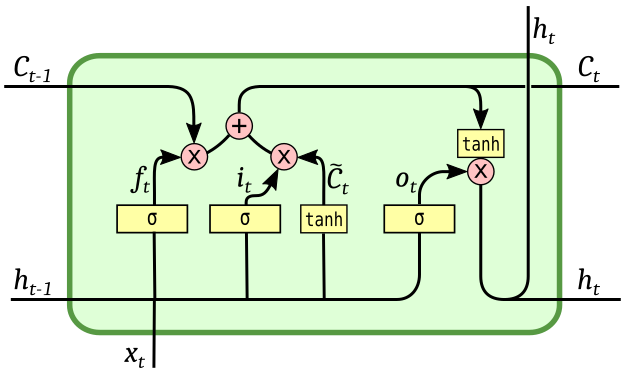
\includegraphics[height=1.5in, width=2.44in]{lstm2.png}
        \caption{The LSTM Cell}
        \end{figure}
      \end{column}

      \end{columns}
      \vspace*{2em}

      \tiny
      Mikolov, Toma's. Statistical Language Models Based on Neural Networks. Ph.D. thesis, Brno University of Technology.(2012)

      Zaremba, Wojciech, I. Sutskever, and O. Vinyals. Recurrent Neural Network Regularization. Eprint Arxiv (2014).
    \end{frame}

    \begin{frame}{Attention weight}
      \begin{columns}
      \begin{column}[t]{0.5\textwidth}
        \begin{figure}
        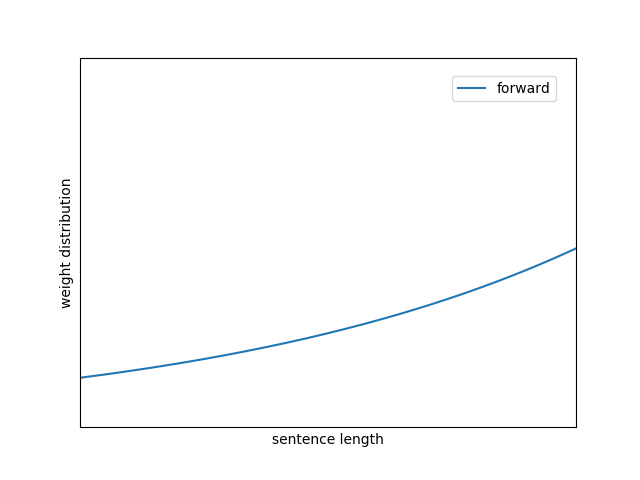
\includegraphics[width=6.4cm,height=4.8cm]{forward.png}
        \caption{Unidirectional weight distribution}
        \end{figure}
      \end{column}

      \begin{column}[t]{0.5\textwidth}
        \begin{figure}
        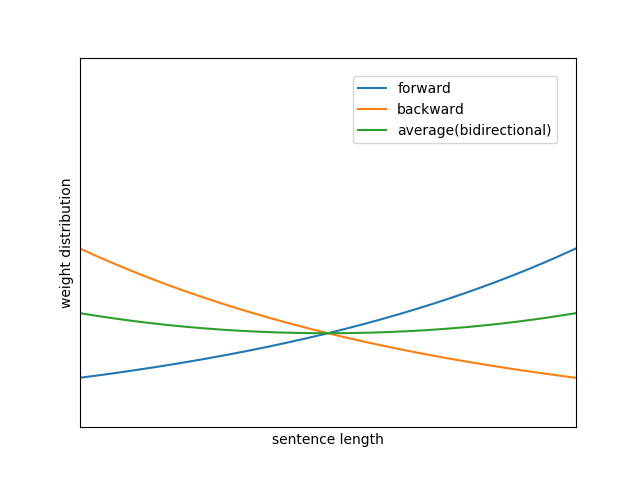
\includegraphics[width=6.4cm,height=4.8cm]{bidirectional.png}
        \caption{bidirectional weight distribution}
        \end{figure}
      \end{column}

      \end{columns}
    \end{frame}

    \begin{frame}{LSTM-Sen2Vec}
      \begin{columns}
      \begin{column}[t]{0.5\textwidth}
        \begin{figure}
        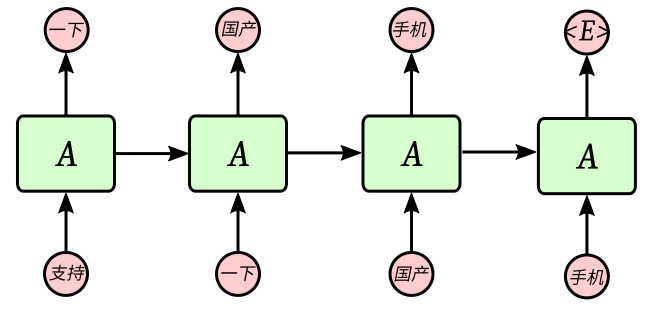
\includegraphics[width=6.7cm,height=3.2cm]{unilstm.png}
        \caption{The Unidirectional LSTM}
        \end{figure}
      \end{column}

      \begin{column}[t]{0.5\textwidth}
        \begin{figure}
        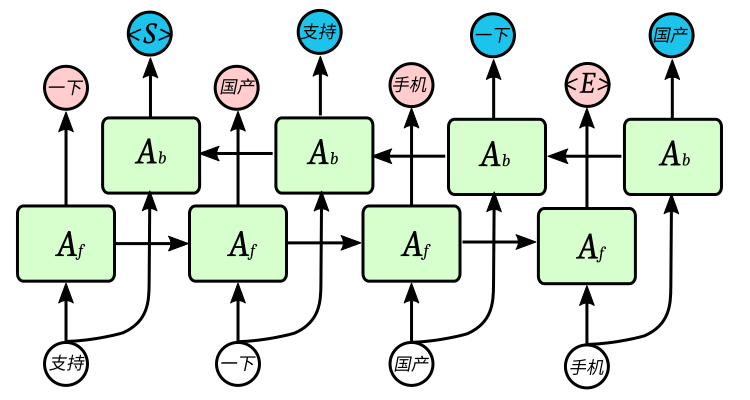
\includegraphics[width=6cm,height=3.2cm]{bilstm1.png}
        \caption{The Traditional Bidirectional LSTM}
        \end{figure}
      \end{column}

      \end{columns}
    \end{frame}

    \begin{frame}{LSTM-Sen2Vec}
      \begin{figure}
        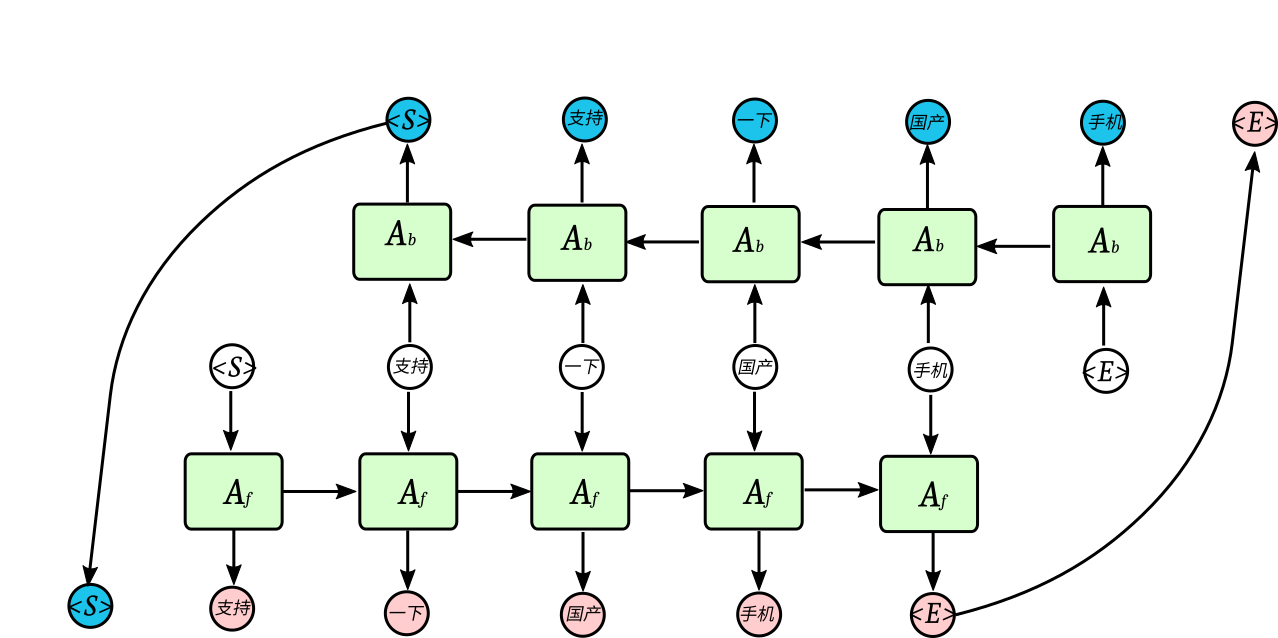
\includegraphics[width=12cm,height=6cm]{bilstm2.png}
        \caption{The Modified Bidirectional LSTM}
        \end{figure}
    \end{frame}

    \begin{frame}{Candidates Generation}
      \begin{itemize}
      \item Similar Posts
      \begin{equation}
         Score_{q,p}^1(q, p) = Sim_{LDA}(q, p) * Sim_{W2V}(q, p) * Sim_{LSTM}(q, p)
      \end{equation}
      \begin{equation}
         Score_{q,p}^2(q, p) = Sim_{LSA}(q, p) * Sim_{W2V}(q, p) * Sim_{LSTM}(q, p)
      \end{equation}
      \item Comment Candidates
      \begin{equation}
         Score_{q,c}^1(q, c) = Sim_{LSA}(q, c) * Sim_{W2V}(q, c)
      \end{equation}
      \begin{equation}
         Score_{q,c}^2(q, c) = Sim_{LDA}(q, c) * Sim_{W2V}(q, c)
      \end{equation}
    \end{itemize}
    \end{frame}

    \begin{frame}{Ranking}
      \begin{itemize}
        \item TextRank (Words as vertices)
        \item Pattern-IDF
        \item Pattern-IDF + TextRank (Sentences as vertices)
      \end{itemize}
    \end{frame}

    \begin{frame}{TextRank - A graph-based ranking model}
      Formally, let $G = (V; E)$ be a undirected graph with the set of vertices 
      $V$ and and set of edges $E$, where $E$ is a subset of $V \times V$. For 
      a given $V_i$, let $link(V_i)$ be the set of vertices that linked with 
      it. The score of a vertex $Vi$ is define as follow:
      \begin{equation}
        WS(V_i) = (1 - d) + d * \sum_{j \in link(V_i)}{w_{ij} * WS({V_j})}
      \end{equation}
      Where $d$ is a damping factor\footnotemark that is usually set to 0.85.

      \footnotetext{Brin, Sergey, and L. Page. The anatomy of a large-scale hypertextual Web search engine. International Conference on World Wide Web Elsevier Science Publishers B. V. 1998:107-117.}
    \end{frame}

    \begin{frame}{TextRank - Vertices and Edges}
      \begin{itemize}
        \item Vertices: each unique word in candidates
        \item Edges: a co-occurrence relation
        \item Weighted by: word2vec similarity between two words and the number of their cooccurrences
      \end{itemize}
    \end{frame}

    \begin{frame}{TextRank - Calculate Iteratively}
      For $N$ candidates, $k$ words in total, we construct $ k \times k $ 
      matrix $M$. $M_{ij} = cnt * sim(D_i, D_j)$. Then we compute iteratively
      \[
      R(t+1) = 
      \begin{bmatrix}
          (1-d)/k       \\
          (1-d)/k       \\
          \hdotsfor{1} \\
          (1-d)/k       
      \end{bmatrix}
      +d
      \begin{bmatrix}
          M_{11} & M_{12} & M_{13} & \dots  & M_{1k} \\
          M_{21} & M_{22} & M_{23} & \dots  & M_{2k} \\
          \vdots & \vdots & \vdots & \ddots & \vdots \\
          M_{k1} & M_{k2} & M_{k3} & \dots  & M_{kk}
      \end{bmatrix}
      R(t)
      \]
      %$R(0) = [IDF(D_0) \ IDF(D_1) \ ... \ IDF(D_{k-1})]^T$ \newline
      Stop when $|R(t+1)-R(t)|<\epsilon$, $\epsilon = 10^{-7}$. \\
      Here, $cnt$ refers to the number of co-ocurrences within a sentence for $D_i$ and $D_j$. \\
    \end{frame}

    \begin{frame}{TextRank - Ranking}
      Since we get the score $R(D_i)$ for each word $D_i$ in candidates, the 
      score for each comment candidate $c$ is calculated as:
      \begin{equation}
        Rank_{TextRank}(c) = \frac{\sum_{D_i \in c}{R(D_i)}}{len(c)} 
      \end{equation}
      Here, $len(c)$ refers to the number of words in comment c.
    \end{frame}

    \begin{frame}{Pattern-IDF}
      For word $D_i$ (minor word) in corresponding comment given word $D_j$ (major word) in the post, we define ($D_j$,$D_i$) as a pattern.

      Inspired by the IDF, we calculate the Pattern-IDF as:
      \begin{equation}
        PI(D_i|D_j) = 1 / \log_2{\frac{count_c(D_i) * count_p(D_j)}{count_{pair}(D_i, D_j)}}
      \end{equation}
      Here $count_c$ refers to the number of occurrence in comments, $count_p$ in posts, $count_{pair}$ in post-comment pair. The PI whose $count_{pair}(D_i, D_j)$ less than 3 are eliminated.

    \end{frame}

    \begin{frame}{Pattern-IDF}
      Let $X = \frac{count_c(D_i) * count_p(D_j)}{count_{pair}(D_i, D_j)}$, then $X \in [1, \infty)$.
      \begin{columns}[T] % align columns
      \begin{column}{.48\textwidth}
      
      \begin{figure}
      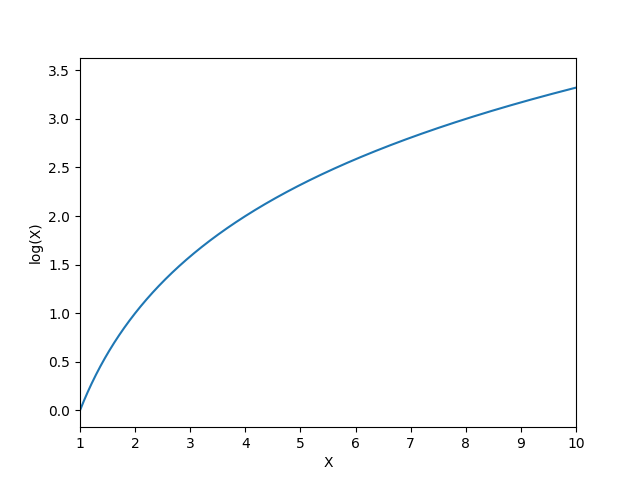
\includegraphics[width=6.4cm,height=4.8cm]{pi1.png}
      \caption{log(X)}
      \end{figure}
      
      \end{column}%
      \hfill%
      \begin{column}{.48\textwidth}
      
        \begin{figure}
        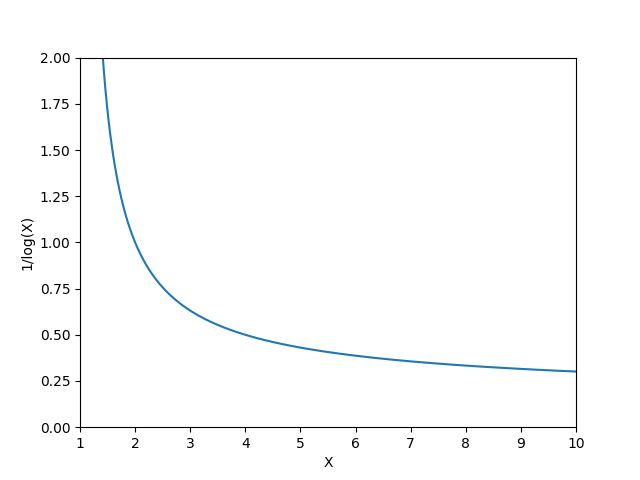
\includegraphics[width=6.4cm,height=4.8cm]{pi2.png}
        \caption{1/log(x)}
        \end{figure}

      \end{column}%
      \end{columns}
    \end{frame}

    \begin{frame}{PI - Example}
      \begin{columns}[T] % align columns
      \begin{column}{.48\textwidth}
      \begin{table}[small]
        \centering
        \caption{The example of Pattern-IDF}
        \resizebox{\linewidth}{!}{% Resize table to fit within \linewidth horizontally
        \begin{tabular}{lll}
        \hline
         $Major Word$ & $Minor Word$ & $PI$ \\ \hline
         中国移动 (China Mobile) & 接通 (connect)   & 0.071725 \\ \hline
         中国移动 & cmcc                                  & 0.067261 \\ \hline
         中国移动 & 资费 (charges)   & 0.062408 \\ \hline
         中国移动 & 营业厅 (business hall
        ) & 0.059949 \\ \hline
         中国移动 & 漫游 (roamimg)   & 0.059234 \\ \hline
         ... & ...  & ...  \\ \hline
         中国移动 & 我 (me)   & 0.028889 \\ \hline
         中国移动 & 是 (be)   & 0.027642 \\ \hline
         中国移动 & 的 (of)   & 0.026346 \\ \hline
        \end{tabular}}
        \end{table}

      
      \end{column}%
      \hfill%
      \begin{column}{.48\textwidth}
      \begin{table}[small]
        \centering
        \caption{The entropy of Pattern-IDF for each Major Word}
        \resizebox{.65\linewidth}{!}{% Resize table to fit within \linewidth horizontally
        \begin{tabular}{ll}
        \hline
         $Major Word$   & H \\ \hline
         眼病  (eye disease)     & 0.889971 \\ \hline
         丰收年 (harvest year)      & 0.988191 \\ \hline
         血浆 (plasma)            & 1.033668 \\ \hline
         脊椎动物 (vertebrate)    &  1.083438 \\ \hline
         水粉画 (gouache painting)&  1.180993 \\ \hline
         ...            & ...        \\ \hline
         现在 (now)     & 9.767768   \\ \hline
         什么 (what)  & 10.219045  \\ \hline
         是 (be)         & 10.934950   \\ \hline
        \end{tabular}}
        \end{table}

        
      \end{column}%

      \end{columns}
      
      \begin{equation}
      \Fontvi
      PI_{norm}(D_i|D_j) = \frac{PI(D_i|D_j)}{\sum_{i=1}^n{PI(D_i|D_j)}}
      \end{equation}
      \begin{equation}
      \Fontvi
      H(D_j) = - \sum_{i=1}^n{PI_{norm}(D_i|D_j)\log_2{PI_{norm}(D_i|D_j)}}
      \end{equation}

    \end{frame}

    \begin{frame}{PI - Ranking}
      For each comment $c$ in candidates, given a query (new post) $q$, we 
      calculate the score by $PI$ as follow:
      \begin{equation}
        Score_{PI}(q, c) = \frac{\sum_{D_j \in q}{\sum_{D_i \in c}{PI(D_i|D_j)}}}{len(c) * len(q)}
      \end{equation}
      Then we define rank score as follow:
      \begin{equation}
        Rank_{PI} = (1 + \frac{Score_{PI}(q, c)}{\max{Score_{PI}(q, c)}}) * Sim_{W2V}(q, c)*Sim_{LSA}(q, c)  
      \end{equation}
    \end{frame}

    \begin{frame}{TextRank + Pattern-IDF}
      In this method, We add each comment sentence in candidates as a vertex in the graph and use sentence Word2Vec similarity as edges between vertices in the graph.

      For $N$ candidates, we construct $ N \times N $ matrix $M$. $M_{ij} = Sim_{w2v}(candidate_i, candidate_j)$. 

      At time $t = 0$, We initiate a N-dimension vector $P$ , here $N$ is the number 
      of comment candidates. And each entry of $P$ is defined as the score of Pattern-IDF between the query (new post) $q$ and corresponding comment $c_i$ in candidates:
      \begin{equation}
        P_i = Score_{PI}(q, c_i)
      \end{equation}
    \end{frame}

    \begin{frame}{TextRank + Pattern-IDF}
      Then we compute iteratively
      \[
      R(t+1) = 
      \begin{bmatrix}
          (1-d)/N       \\
          (1-d)/N       \\
          \hdotsfor{1} \\
          (1-d)/N       
      \end{bmatrix}
      +d
      \begin{bmatrix}
          M_{11} & M_{12} & M_{13} & \dots  & M_{1N} \\
          M_{21} & M_{22} & M_{23} & \dots  & M_{2N} \\
          \vdots & \vdots & \vdots & \ddots & \vdots \\
          M_{N1} & M_{N2} & M_{N3} & \dots  & M_{NN}
      \end{bmatrix}
      R(t)
      \]
      Stop when $|R(t+1)-R(t)|<\epsilon$, $\epsilon = 10^{-7}$

      Finally, we get the score $P_i$ for each comment in candidates. 
    \end{frame}

  \begin{frame}{Experiment}
    \begin{itemize}
      \item{Nders-C-R5: } LDA + Word2Vec + LSTM-Sen2Vec 
      \item{Nders-C-R4: } LSA + Word2Vec + LSTM-Sen2Vec 
      \item{Nders-C-R3: } R4 + TextRank (Words as vertices)
      \item{Nders-C-R2: } R4 + Pattern-IDF 
      \item{Nders-C-R1: } R4 + Pattern-IDF + TextRank (Sentences as vertices)
    \end{itemize}
  \end{frame}

  \begin{frame}{Official Result}
    \begin{table}
\centering
\caption{The official results of five runs for Nders team}
\label{tab:commands}
\begin{minipage}{\columnwidth}
\begin{center}
\begin{tabular}{|l|c|c|c|}
\hline
 Run        &  Mean nG@1  &  Mean P+  &  Mean nERR@10  \\ \hline
 Nders-C-R1 & 0.4593 & 0.5394 & 0.5805 \\ \hline
 Nders-C-R2 & 0.4743 & \textbf{0.5497} & \textbf{0.5882} \\ \hline
 Nders-C-R3 & 0.4647 & 0.5317 & 0.5768 \\ \hline
 Nders-C-R4 & \textbf{0.4780} & 0.5338 & 0.5809 \\ \hline
 Nders-C-R5 & 0.4550 & 0.5495 & 0.5868 \\ \hline
 \textcolor{red}{R2 \ vs. \  R4}  & \textcolor{red}{$\downarrow$0.77\%} & \textcolor{red}{$\uparrow$2.98\%} & \textcolor{red}{$\uparrow$1.26\%} \\ \hline

\end{tabular}
\end{center}
\end{minipage}
\end{table}
  \end{frame}

  \begin{frame}[standout]
    Questions?
  \end{frame}

\end{document}

